%%%%%%%%%%%%%%%%%%%%%%%%%%%%%%%%%%%%%%%%%%%%%%%%%%%%%%%%%%%%%%%%%%%%%%%%%%%%%%%%
%2345678901234567890123456789012345678901234567890123456789012345678901234567890
%        1         2         3         4         5         6         7         8

\documentclass[letterpaper, 10 pt, conference]{ieeeconf}  % Comment this line out
                                                          % if you need a4paper
%\documentclass[a4paper, 10pt, conference]{ieeeconf}      % Use this line for a4
                                                          % paper

\IEEEoverridecommandlockouts                              % This command is only
                                                          % needed if you want to
                                                          % use the \thanks command
\overrideIEEEmargins
% See the \addtolength command later in the file to balance the column lengths
% on the last page of the document


\usepackage{subfigure}
\usepackage{graphicx}
% The following packages can be found on http:\\www.ctan.org
\usepackage{graphics} % for pdf, bitmapped graphics files
\usepackage{epsfig} % for postscript graphics files
%\usepackage{mathptmx} % assumes new font selection scheme installed
%\usepackage{times} % assumes new font selection scheme installed
\usepackage{amsmath} % assumes amsmath package installed
%\usepackage{amssymb}  % assumes amsmath package installed
\usepackage{listings}
\usepackage{booktabs}
\usepackage{cite}
\usepackage{float}
%\usepackage{hyperref}
\usepackage{footmisc}
\usepackage[vlined,boxed,commentsnumbered,ruled]{algorithm2e}
\usepackage{array}
\usepackage{algorithmic}

\title{\LARGE \bf
Monocular Visual Localization using Road Structural Features
}

\author{Yufeng Yu$^{*}$, Huijing Zhao$^{*}$, Jinshi Cui$^{*}$, Hongbin Zha$^{*}$, Franck Davoine$^{+}$
\thanks{$^{*}$Y. Yu, H. Zhao, J. Cui and H. Zha are with the State Key Lab of Machine Perception (MOE), Peking University, Beijing, China. {\tt\small yuyufeng at pku.edu.cn}}
\thanks{$^{+}$F. Davoine is with CNRS, LIAMA Sino French Laboratory, Beijing, China}%
}


\begin{document}
\maketitle
\thispagestyle{empty}
\pagestyle{empty}


\begin{abstract}

Precise localization is an essential issue for autonomous driving applications, where GPS-based localization systems have challenges in meeting the requirements such as lane-level accuracy. This research studies a visual-based approach on structured roads using a monocular camera, where a major focus is to improve robustness of a visual localization algorithm in dynamic traffic environments. Concerning that in a structured road environment, the line features on lane markings, curbs, poles, building edges, etc. are dominant, which demonstrate the road's longitude, latitude and vertical directions, a road structural feature (RSF) is defined as a set of line segments with direction of three perpendicular axes together with some feature points. A RSF-based visual localization method is proposed, where a prior knowledge of the environment, such as a 2D map with road-direction information, is implemented in a map-based localization framework, which predicts a RSF (or multiple RSFs at intersections) of the scene, and then estimates vehicle pose with the RSFs. Experiments have been conducted using the video streams that were collected on major roads in central Beijing, which are structured and dynamic. GPS/IMU data were collected and synchronized with the video streams as a reference in validation. The result shows better performance compared with that of a tradition visual odometry method. Future work will be addressed on using visual approach to improve GPS localization accuracy.
\end{abstract}

\section{Introduction}
For decades, there have been enormous research efforts in developing autonomous/assisted driving and mobile mapping systems \cite{urmson2008autonomous}. An essential issue of these systems is precise localization of a vehicle platform in a real world traffic environment, where approaches using different sensors have been studied extensively.

GPS (Global Positioning System) has been widely used in car navigation systems, which visualize the car's location on a map or guide the car's route to assist for human drivers' decision making.
However, for the applications such as autonomous driving, GPS-based localizations have many challenges.
GPS signals could be obstructed by bridges, tunnels, buildings, etc., and its accuracy could be greatly degraded due to the multi-path problem especially in a downtown area. Although an IMU (Inertial Measure Unit) can be used to interpolate position during the period of GPS outage \cite{caron2006gps}, while its accuracy maintains only for short periods due to the accelerometer biases and gyro drifts.
More importantly, an autonomous vehicle needs to find its location on road lanes, e.g. if the vehicle will make a right turn, it needs to be or change to the rightmost lane, etc., while the state-of-the-art GPS-based localization systems can not provide at lane-level accuracy. It is thus of great demand on developing localization approaches using on-board high dimensional sensors, such as a LiDAR (Light Detection and Ranging), a mono camera or a stereo vision system.

This research studies a visual-based approach to achieve precise localization at structured road environments using a monocular camera, where high dynamic traffic is one of the greatest challenges.
As in a structured road environment, the line features on lane markings, curbs, poles, building edges, etc. are dominant, which demonstrate the road's longitude, latitude and vertical directions.
A new feature, named road structural feature (RSF), is extracted from the set of line segments, which characterize such a typical property of a structured road environment using the three perpendicular axes at a local road frame together with the feature points.
A RSF-based visual localization method using a monocular camera is proposed, where a prior knowledge to the environment, such as a rough map with skeleton road structure, is implemented in a map-based localization framework, which predicts a RSF (or multiple RSFs at intersections) of the scene, and vehicle pose is estimated after detecting the RSF from a monocular image with the predictions.
Experiments have been conducted using the video streams that were collected on major roads in central Beijing, which are structured and dynamic. In this particular work, GPS/IMU data were collected and synchronized with the video streams as a reference in validation, while future work will be addressed on a fusion-based system that using visual approach to improve GPS localization accuracy.

The paper is organized as follows. A review to the state-of-the-art localization approaches using on-board high dimensional sensors as well as an analysis of the major challenges is given in section II. An overview of the system is presented in section III. The details of RSF-based localization are addressed in section IV. Experimental results are demonstrated and discussed in section V, followed by conclusion and future works in Section VI.

\section{Background}

The high dimensional sensor, such as a LiDAR (Light Detection and Ranging), a mono camera or a stereo vision system, has been studied to find vehicle pose, the problem of which falls into the realm of SLAM (Simultaneous Localization And Mapping) \cite{durrant2006simultaneous}. LiDAR is an active sensor measuring range distances by estimating the TOF (Time-Of-Flight) of laser beams to surrounding objects. A 2D LiDAR that scanning at a horizontal plane is well used to localize a robot at a flat area \cite{zhang2000line}. 3D LiDAR has also been studied to find 6DOF localization \cite{moosmann2011velodyne}, while the high cost or long scanning period put many restrictions on its real applications. Estimating a platform's motion using visual input is also known as visual odometry or visual localization \cite{nister2004visual}. Due to the low cost and diversity of camera sensors, high frequency and capability of 3D localization, visual odometry has been applied on many different kinds of systems.
Estimating robot motion using visual odometry can be traced back to \cite{moravec1980obstacle}. Good results are found in \cite{nister2004visual}. After that, many researchers are doing improvements based on basic visual odometry algorithm. Mouragnon \emph{et al}.\cite{mouragnon2006real} introduced a fast local bundle adjustment method, which made the result more accurate and consistent. Parra \emph{et al}.\cite{parra2011visual} fused a stereo-vision based visual odometry with map data for GPS navigation assistance, which kept track of the vehicle position on a road of a digital map. Ramalingam \emph{et al}.\cite{ramalingam2011pose, ramalingam2010skyline2gps} used the 3D model of the city to get the correspondence between the 2D image space and 3D world space. The results were excellent, but a good city model was needed.

%Estimating robot motion using visual odometry can be traced back to [Moravec 1980]. Good results are found in [select some representative works, e.g. Matthies and Shafer 1987, Kriegman, Triendl and Binford 1989, Zhang, Faugeras and Ayache 1988, Lacroix et al. 1999, Mallet, Lacroix and Gallo 2000, Jung and Lacroix 2005, Maimone et al. 2004, Nister 2006). However few of the existing approaches address the challenges in a dynamic traffic environment, such as an urban street.

\begin{figure}
\centering
 \begin{minipage}[t]{0.48\linewidth}
    \centering
    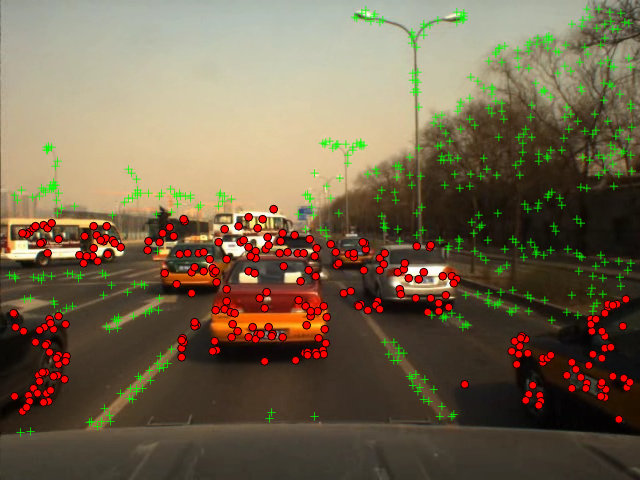
\includegraphics[width=1\textwidth]{source//Final//image0130_277in785.png}
    \label{fig:line_feature}
  \end{minipage}%
  \hfill
 \begin{minipage}[t]{0.48\linewidth}
    \centering
    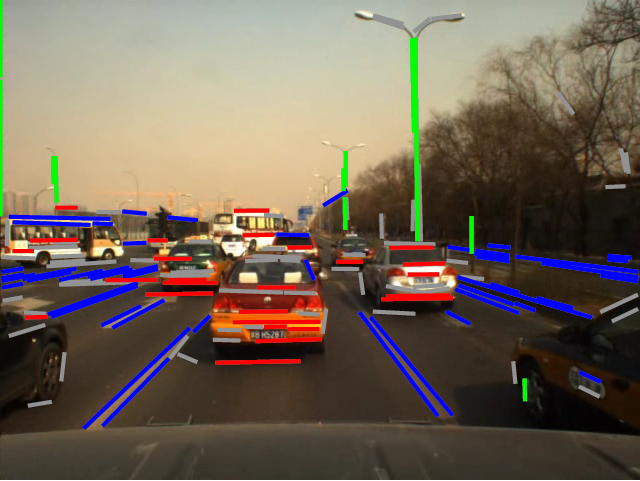
\includegraphics[width=1\textwidth]{source//Final//image0130_84in144.png}
    \label{fig:point_feature}
  \end{minipage}%
 \vfill
 \begin{minipage}[t]{0.48\linewidth}
    \centering
    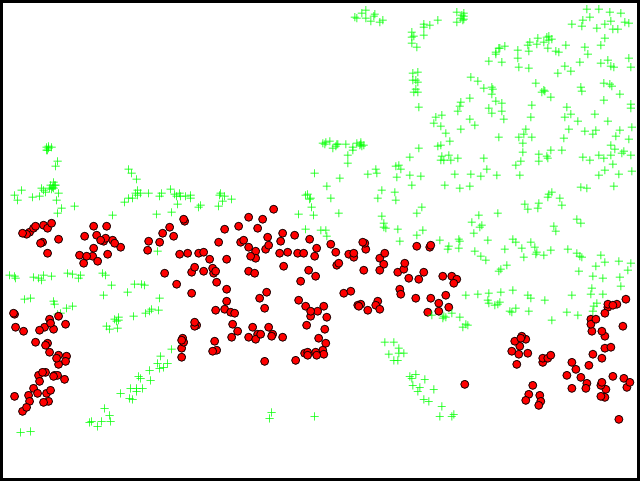
\includegraphics[width=1\textwidth]{source//Final//image0130_277in785_blank.png}
    \label{fig:line_in_blank}
  \end{minipage}%
  \hfill
 \begin{minipage}[t]{0.48\linewidth}
    \centering
    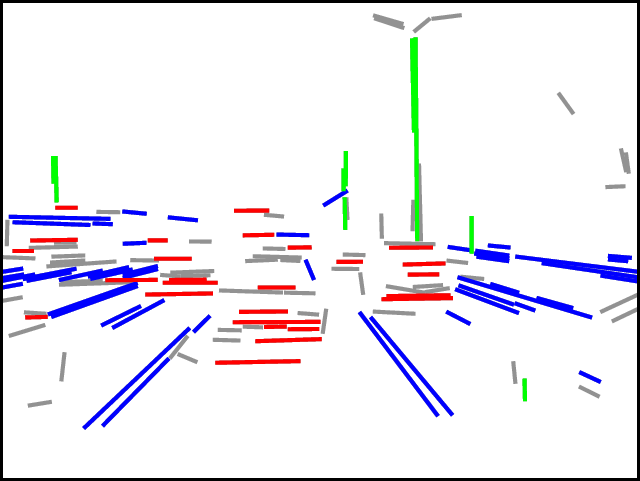
\includegraphics[width=1\textwidth]{source//Final//image0130_84in144_blank.png}
    \label{fig:point_int_blank}
  \end{minipage}%
  \vfill
 \begin{minipage}[t]{0.48\linewidth}
    \centering
    (a)
  \end{minipage}%
  \hfill
 \begin{minipage}[t]{0.48\linewidth}
    \centering
    (b)
  \end{minipage}%
\caption{Different features detected from a certain frame. Pictures in column (a) show the point features detected using optical flow. The points in red or green are detected on the moving or static objects. Pictures in column (b) show the line features detected using LSD (Line Segment Detector) \cite{von2012lsd}. The line segments in blue, red and green demonstrate the road's longitude, latitude and vertical directions.}
\label{fig:features}
\end{figure}

The utmost of a visual odometry system is a feature tracker, where feature extraction and correlation are essential to vehicle pose estimation. Many methods detect and match the feature points of successive frames for localization. And in order to rule out the interference from dynamic objects, RANSAC (Random Sample Consensus) \cite{fischler1981random} is usually applied. However, as the number of moving objects increases as the example shown in Fig. \ref{fig:features}(a), where among the 785 feature points, 277 come from surrounding cars, it becomes extremely difficult in discriminating outliers and finding a reliable estimation to vehicle pose. Although Kundu \emph{et al}.\cite{kundu2011realtime}  implemented motion segmentation to remove the interference of surrounding moving objects in estimating ego-vehicle's pose, reliable motion segmentation in a high dynamic traffic scene is still an open problem.
Compared with point features, line features are dominant in a structured road environment. As shown in the column of Fig. 1 (b), the line segments in blue, red and green represent the road's longitude, latitude and vertical directions composing a local road frame.
From these set of line segments, three perpendicular axes relative to the road can be extracted. With such a feature, the surrounding cars are no longer interference factors, the line segments on environmental cars provide additional supports, which could be used to infer the rotation from ego-vehicle to a road frame.
So a new feature named road structural feature is defined as a set of line segments with direction of three perpendicular axes relative to the road together with feature points, which can be used for localization in a dynamic traffic environment.

\section{System Outline}

\begin{figure}
\centering
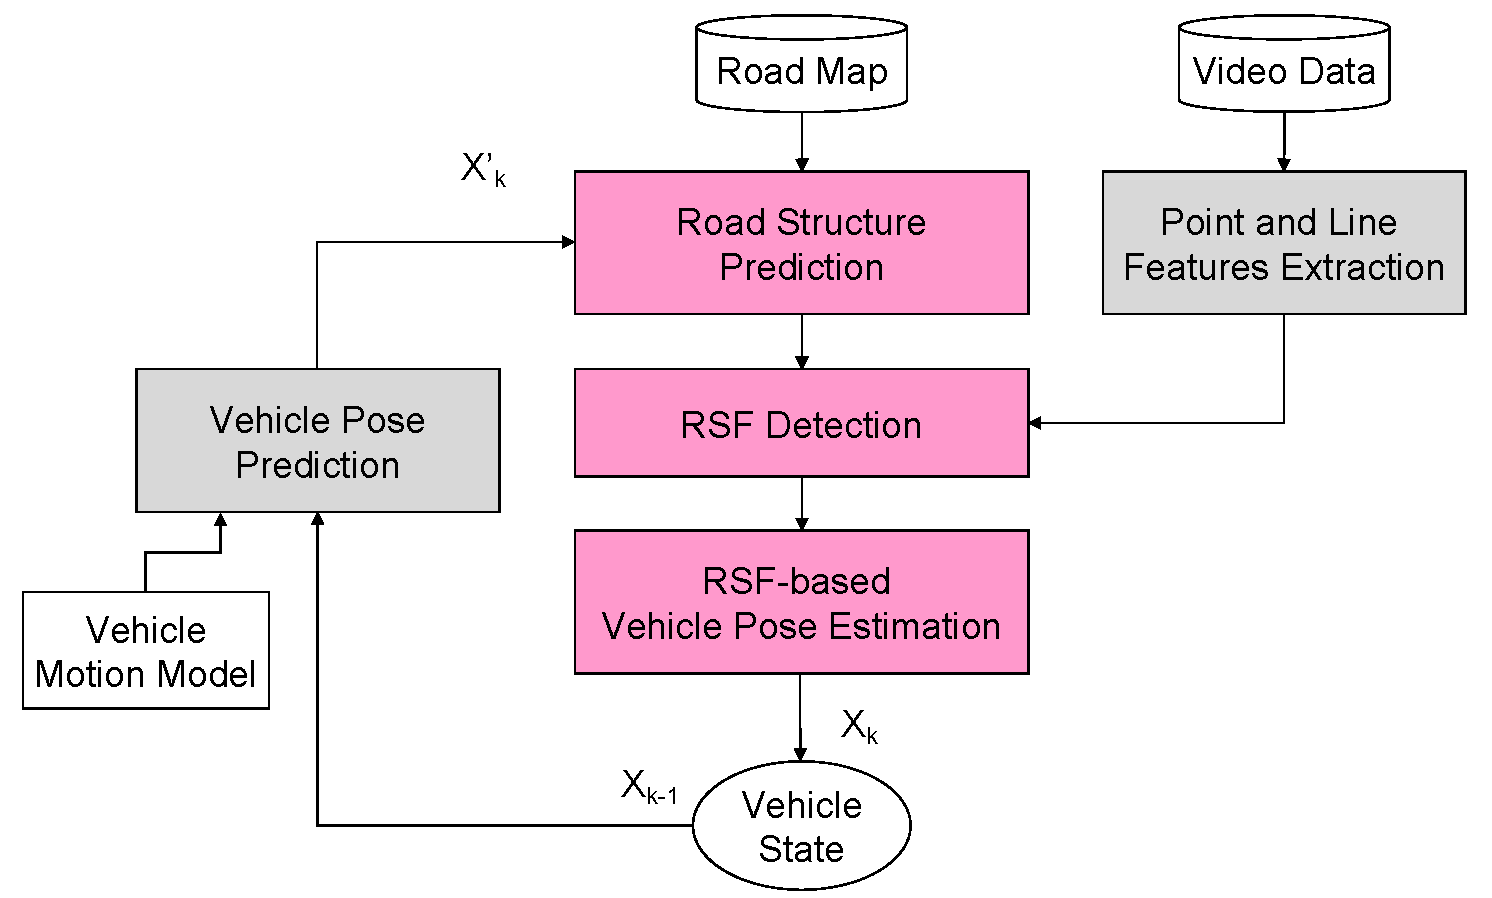
\includegraphics[width=0.9\linewidth]{source//Final//framework.pdf}
\caption{System framework. The key point is to define RSF and use it to calculate the vehicle pose.}
\label{fig:framework}
\end{figure}

In this research, a visual-based localization method is proposed by making use of the structural features on broad roads. The system flow is shown in Fig. \ref{fig:framework} consisting of three major steps, i.e. RSF prediction, RSF detection, and RSF-based vehicle pose estimation. They are detailed below.

\begin{figure}
  \centering
  \subfigure[Straight road situation]{
    \centering
    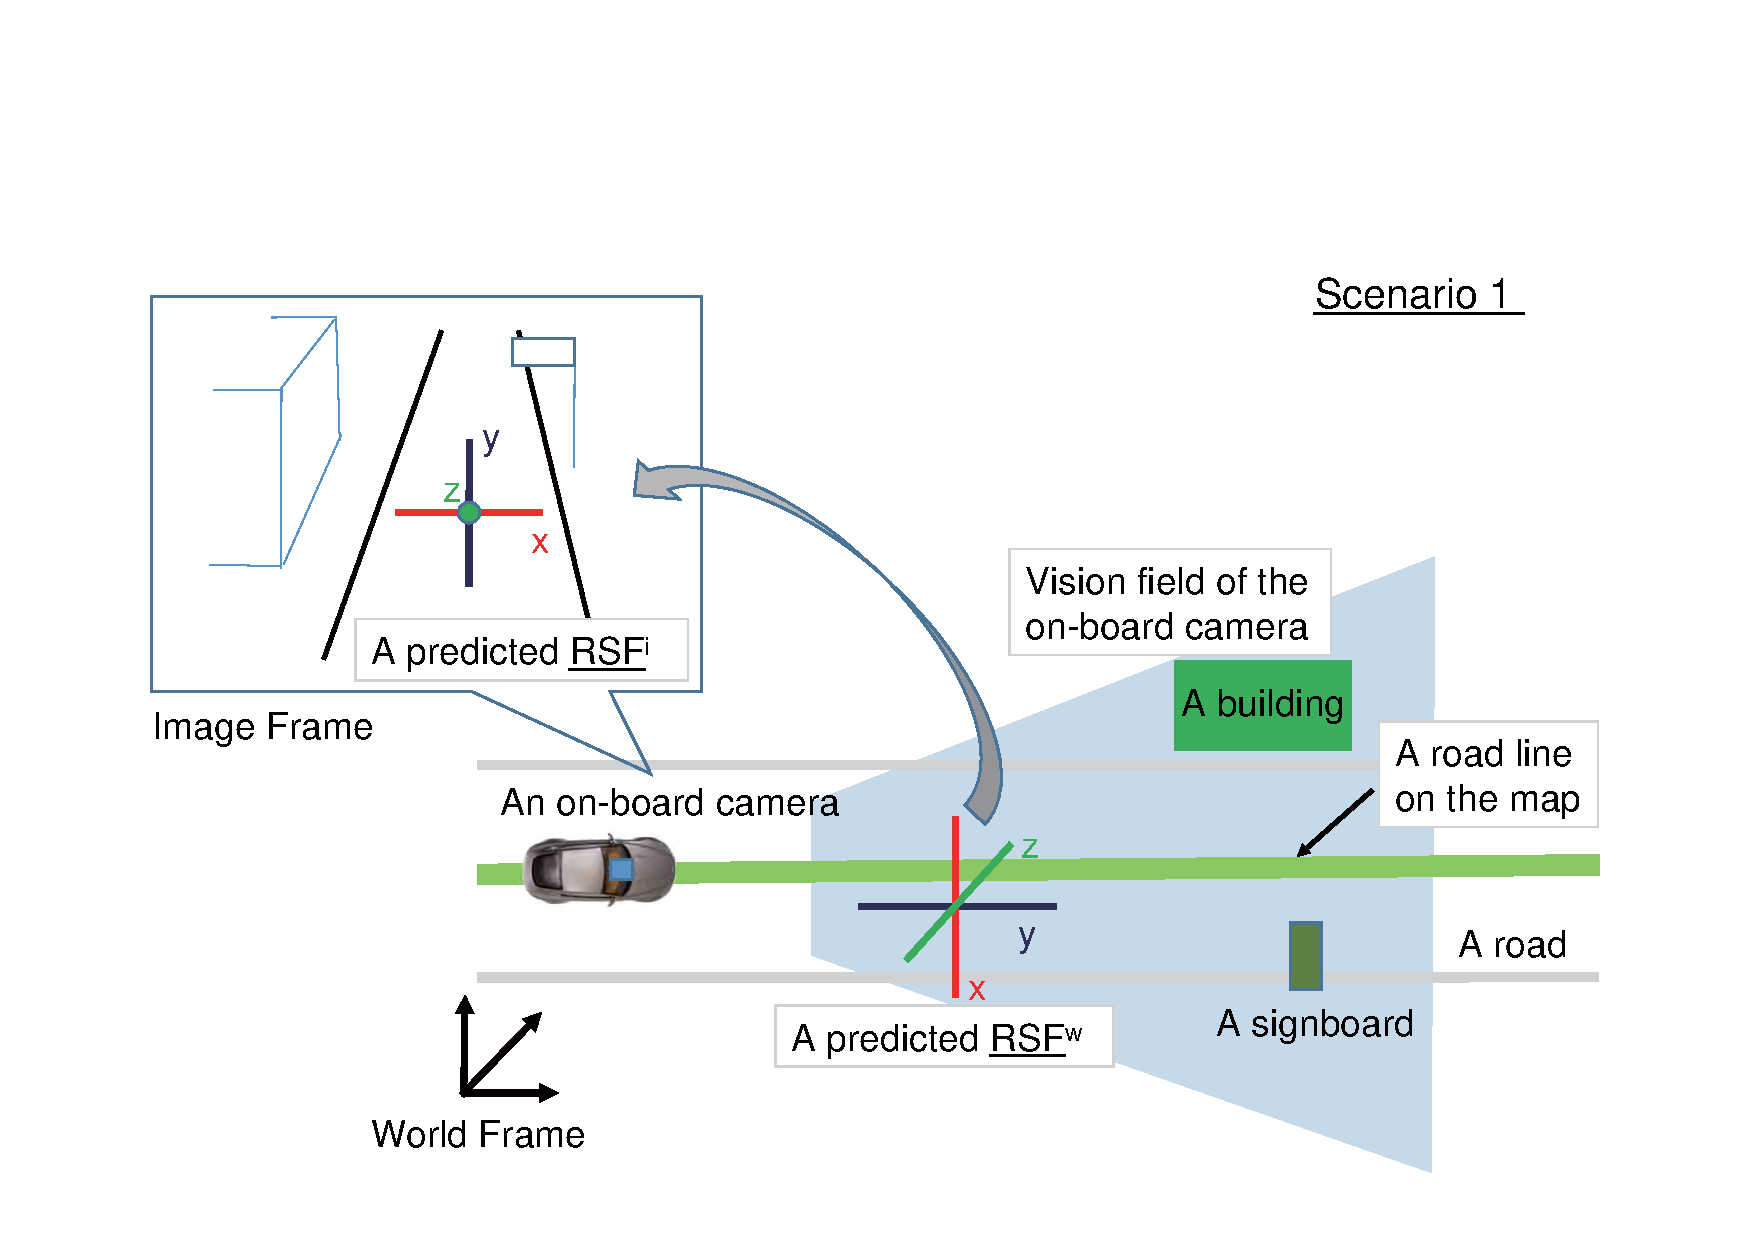
\includegraphics[width=0.9\linewidth]{source//Final//straight_road.pdf}
    \label{fig:straight_road}
  }
  \subfigure[Intersection situation]{
    \centering
    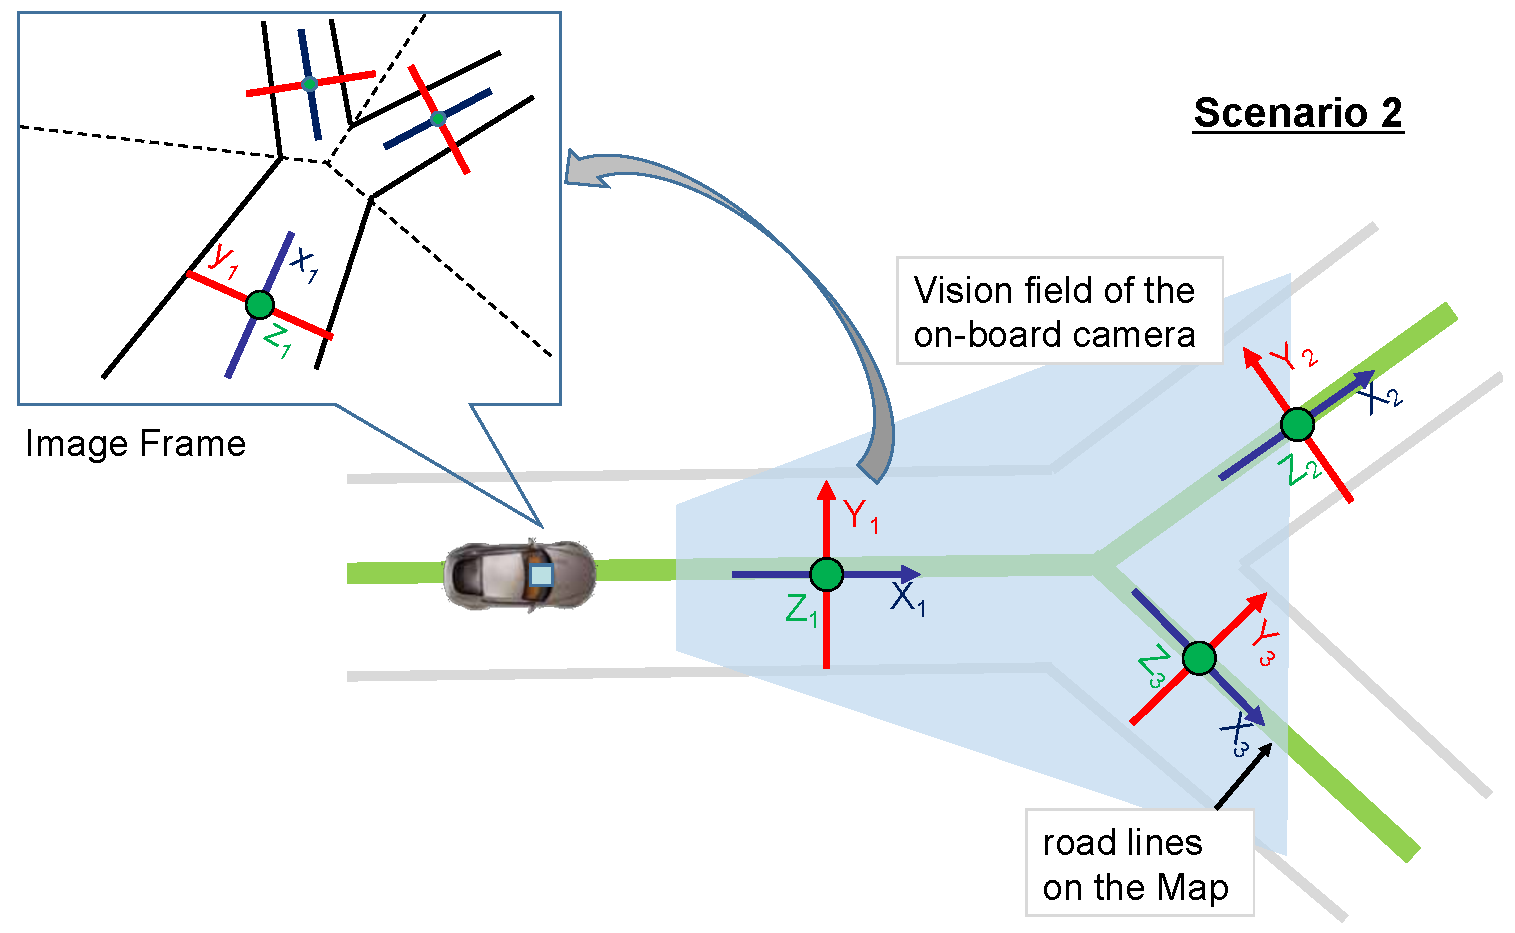
\includegraphics[width=0.9\linewidth]{source//Final//crossing.pdf}
    \label{fig:intersection}
  }
  \caption{Map-based RSF prediction. The road lines are given by the road map, but others like the building and the signboard, are manually added. The light blue trapezium is the camera's field of view and the top-left image is the RSF projection result on the image plane.}
  \label{fig:map_based_prediction}
\end{figure}

\subsubsection{Road structure prediction}
Now a day, many commercial maps are publicly available, such as the OpenStreetMap. With these maps, road lines at a predicted vehicle position are retrieved, and a road structure with three orthogonal axes $\tilde{RS}:\{\mathbf{e}_1,\mathbf{e}_2,\mathbf{e}_3\}$ is subsequently proposed as illustrated in Fig. \ref{fig:map_based_prediction} defining the longitudinal, lateral, and vertical directions of the road. The three orthogonal axes can be further projected onto the image frame according to the extrinsic and intrinsic calibration parameters of the camera, with which the line features are selected and discriminated in the next step. At an intersection scene, several $\tilde{RS}$s are predicted in similar ways, and the image frame is subsequently partitioned into several zones corresponding to each predicted $\tilde{RS}$ as illustrated in Fig. \ref{fig:intersection}.


\subsubsection{RSF detection}
In this step, a set of visual features $\mathbf{Z}_{RSF}:\{\mathbf{L}_1,\mathbf{L}_2,\mathbf{L}_3,\mathbf{P}\}$ consisting of selected line segments and points is developed, representing the  structural properties of the road. Line segments and feature points of general meaning are first detected from the current image frame using the methods in literature []. With a predicted $\tilde{RS}$, the line segments consistent with the predicted directions of $\mathbf{e}_1$, $\mathbf{e}_2$ and $\mathbf{e}_3$ are selected and classified accordingly into three groups, i.e. $\mathbf{L}_1$, $\mathbf{L}_2$ and $\mathbf{L}_3$, with a distance measure $\mathbf{d}$ that is defined in next section.
The line features on the lane markers and road boundaries along longitudinal road direction are consisted in $\mathbf{L}_1$. Lateral road markings and even the line segmented detected on environmental vehicles contribute to $\mathbf{L}_2$. $\mathbf{L}_3$ contains those from vertical objects, such as poles and buildings. On the other hand, the feature points that are tracked during two succeeding frames are selected in $\mathbf{P}$ at the present stage, while future work will make use of the end points of lane marker, poles by developing corresponding detection methods.


\subsubsection{RSF-based vehicle pose estimation}
A RSF candidate is defined as below, which can be used to estimate a vehicle pose $\mathbf{x}_i$ as detailed in next section.

\begin{equation}
\mathbf{C}_{RSF}=\{\mathbf{l}_1,\mathbf{l}_2\in \mathbf{L}_u, \mathbf{l}_3\in \mathbf{L}_v, u \neq v, \mathbf{p}_1,\mathbf{p}_2\in \mathbf{P}\}
\label{eq:C_RSF}
\end{equation}

Given a set of RSF features $\mathbf{Z}_{RSF}$, a number of candidates $\{\mathbf{C}_{RSF}^i\}$ can be enumerated according to the above definition. Fig. \ref{fig:features_for_estimation} illustrates a type of RSF candidate with $v=1$ and $u=3$, where $\mathbf{l}_1$ and $\mathbf{l}_2$ correspond to longitudinal road boundaries, and $\mathbf{l}_3$ is a vertical edge. Various types of candidates can be generated by changing the values of $u$ and $v$.

With the set of RSF features $\mathbf{Z}_{RSF}$ and candidates $\{\mathbf{C}_{RSF}^i\}$, the problem of vehicle pose estimation at frame $k$ is defined in a probabilistic way as below.

\begin{equation}
\hat{x_k} = \displaystyle \arg\max _{x_k^i \sim \mathbf{C}_{RSF}^i} \{ p(\mathbf{Z}_{RSF} | x_k^i) p(x_k^i|x_{k-1}) \}
\end{equation}

Each vehicle pose $\mathbf{x}_i$ estimated on a candidate $\{\mathbf{C}_{RSF}^i\}$ is evaluated, and the one that yields the maximal posterior of $p(\mathbf{Z}_{RSF} | x_k^i) p(x_k^i|x_{k-1})$ is selected. Here, $p(x_k^i|x_{k-1})$ is estimated in a Gaussian by assuming a linear vehicle motion model.

In the next section, we define a distance measure $\mathbf{d}$ in selecting and classifying the line segments with proposed road axes in RSF detection; detail the algorithm in estimating vehicle pose on a RSF candidate; and present an analytical estimation of the likelihood measure $p(\mathbf{Z}_{RSF} | x_k^i)$ in (2).



\begin{figure}
  \centering
  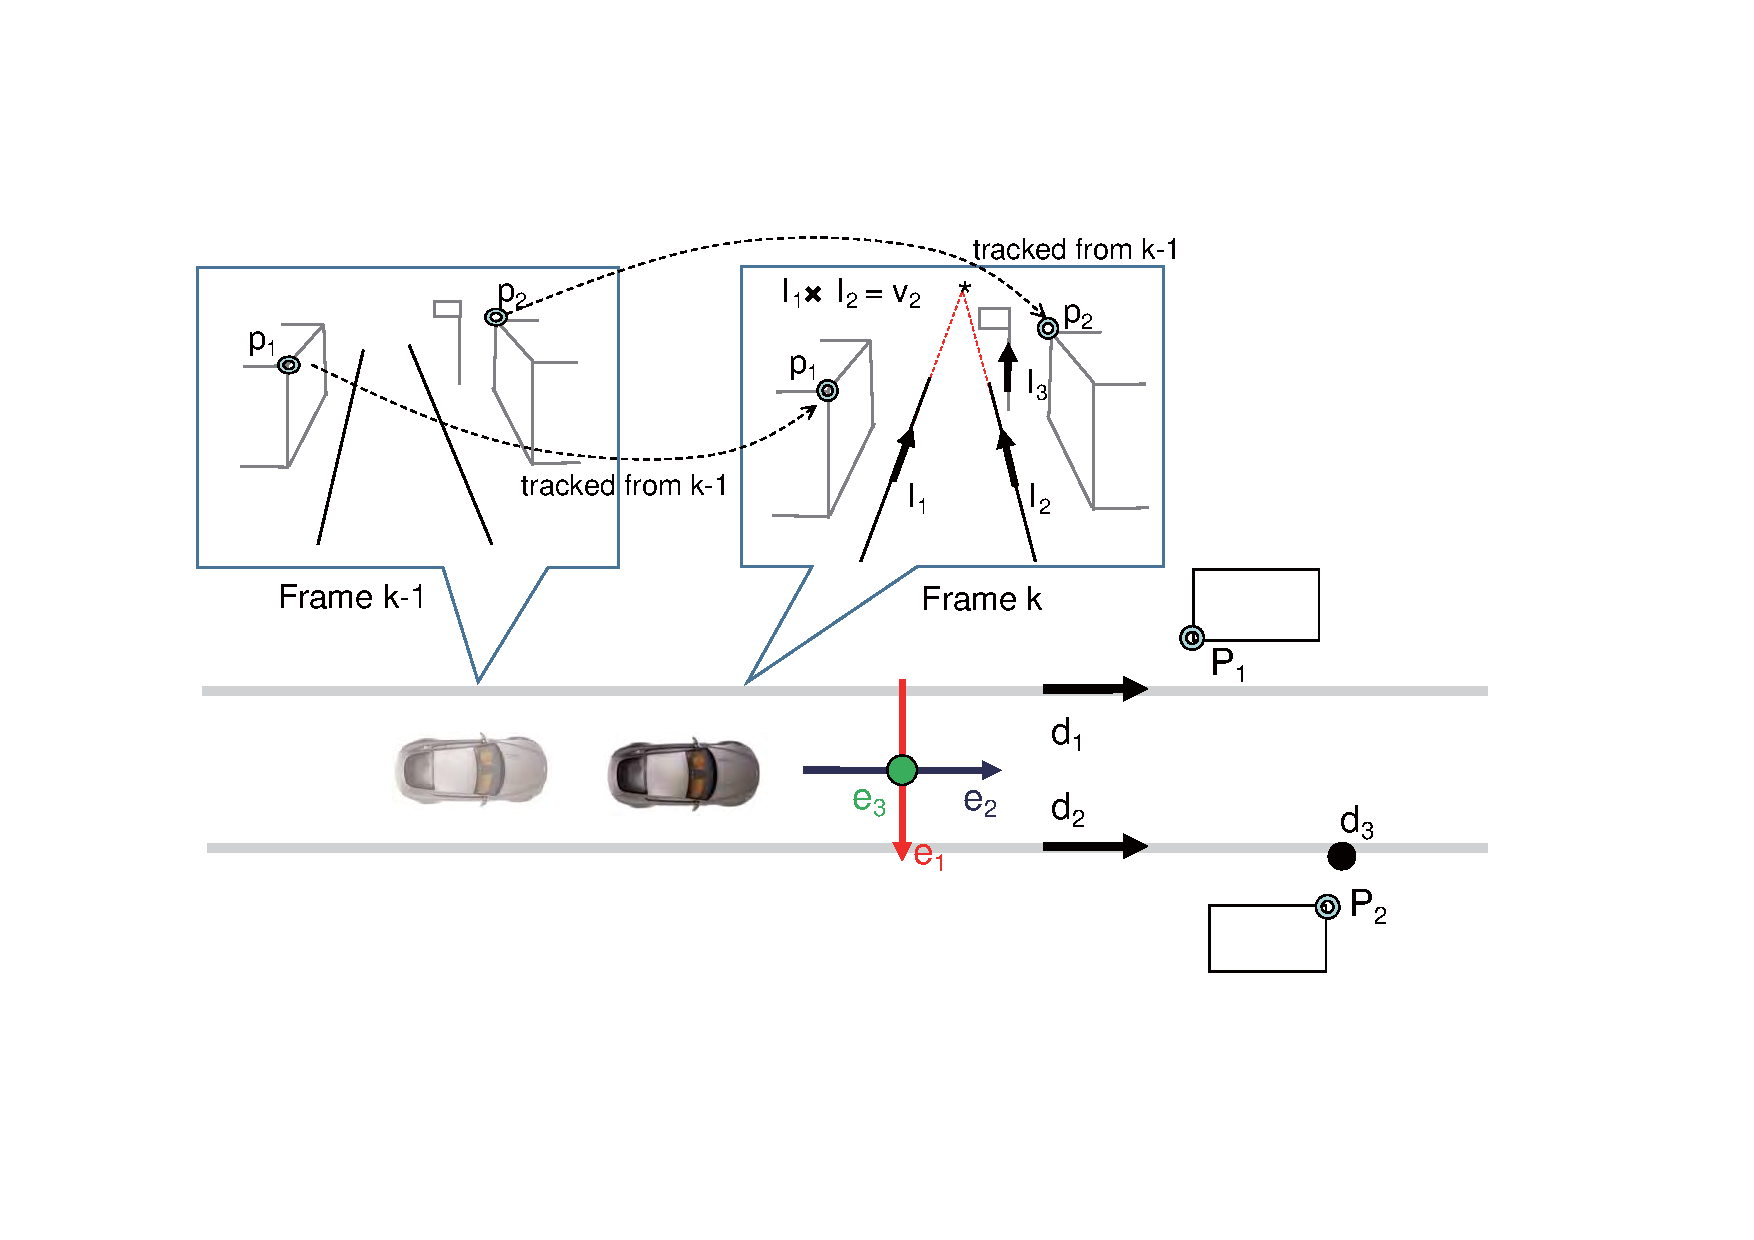
\includegraphics[width=0.9\linewidth]{source//Final//feature.pdf}
  \caption{The features for pose estimation. The line segments detected in a single frame are used for rotation estimation and the points detected and tracked in two frames are used for translation estimation.}
  \label{fig:features_for_estimation}
\end{figure}


\section{Algorithm Details}
%Here the details of the algorithm is presented. The detection of RSF is given in the first place. After that a robust pose estimation algorithm based on RANSAC is explained, followed by the use of the map in RSF or RSFs prediction. Finally, some implementations are presented, which can higher the robustness of the system.

\subsection{Notations and Coordinate Frames}
Before going to the details, Some notations and coordinate frames are presented first. The road coordinate frame is made of the road's longitude, latitude and vertical directions, which are $X_r$, $Y_r$ and $Z_r$. For the vehicle frame, the origin is the center point of the rear axle, $X_v$ is to the right side, $Y_v$ is to the front and $Z_v$ is to the top. For the camera frame, the origin is the center point, $X_c$, $Y_c$ and $Z_c$ are to the left, down and front.

$\mathbf{R}_r$ is the rotation of the road in world coordinate frame calculated by the angle $\theta$, which means
\begin{equation}
\mathbf{R}_r =\begin{bmatrix}   cos\theta & -sin\theta & 0 \\
                                sin\theta & cos\theta & 0 \\
                                0 & 0 & 1
                    \end{bmatrix}
\end{equation}
So the road coordinate is 
\begin{equation}
\begin{bmatrix} \mathbf{X}_r & \mathbf{Y}_r & \mathbf{Z}_r \end{bmatrix}
= \mathbf{R}_r
\begin{bmatrix} \mathbf{e}_1 & \mathbf{e}_2 & \mathbf{e}_3 \end{bmatrix} 
\end{equation}
where $\mathbf{e}_1=(1,0,0)^T$, $\mathbf{e}_2=(0,1,0)^T$, $\mathbf{e}_3=(0,0,1)^T$ are the directions of x,y and z in world coordinate frame.

$\mathbf{x}_{v} = \{\mathbf{R}_{v}, \mathbf{s}_{v}\}$ is the pose of the vehicle, where $\mathbf{R}_v$ is the orientation and $\mathbf{s}_v$ means the position. $\mathbf{x}_{c} = \{\mathbf{R}_{c}, \mathbf{s}_{c}\}$ is the pose of the camera. The coordinate transformation is provided by
\begin{equation}
\mathbf{R}_{c} = \mathbf{R}_v \mathbf{R}_{cv}
\label{eq:R_c}
\end{equation}
\begin{equation}
\mathbf{s}_{c} = \mathbf{s}_v + \mathbf{R}_{v} \mathbf{s}_{cv}
\label{eq:S_c}
\end{equation}
where $\mathbf{R}_{cv}$ and $\mathbf{s}_{cv}$ are the orientation and position of the camera in vehicle coordinate frame, which is well calibrated.

Let $\mathbf{P}=\mathbf{K}[\mathbf{R}|\mathbf{t}]$ is the projection matrix of the camera, where $\mathbf{K}$ is the intrinsic matrix, which is well calibrated, $\mathbf{R}=\mathbf{R}_c^T$ is the rotation matrix, and $\mathbf{t}=-\mathbf{R}_c\mathbf{s}_c$ is the translation vector.

\subsection{Prediction}
The pose of the vehicle $\mathbf{x}_{v,k} = \{\mathbf{R}_{v,k}, \mathbf{s}_{v,k}\}$ in frame $k$ can be predicted by a vehicle motion model. In this paper, the model is assumed to be linear, which means the change of the rotation is linear
\begin{equation}
\hat{\mathbf{R}}_{v,k}=\mathbf{R}_{rel}\mathbf{R}_{v,k-1}=\left(\mathbf{R}_{v,k-1}\mathbf{R}_{v,k-2}^T\right)\mathbf{R}_{v,k-1}
\label{eq:R_t_predict}
\end{equation}

The position is predicted using a linear motion assumption
\begin{equation}
\hat{\mathbf{s}}_{v,k}= \mathbf{s}_{v,k-1} + \hat{\mathbf{d}}_{v,k} \int_{t_{k-1}}^{t_k}{v_t}\,dt
\end{equation}
where $\hat{\mathbf{d}}_k$ is the vehicle's heading provided by $\hat{\mathbf{R}}_{v,k}$, $t_k$ and $t_{k-1}$ are the time of frame $k$ and $k-1$, $v$ is the speed detected from an encoder on the wheel.

Combining (\ref{eq:R_c}) and (\ref{eq:S_c}), the pose of the camera is calculated. Then we get the camera's field of view on the map to find out the direction of the road in a straight road or directions of the roads in the intersection. For the intersection situation, the map projected onto the image and divide the image into several zones for line classification as shown in Fig. \ref{fig:map_based_prediction}.

\subsection{Distance Measure for Line Classification}
To classify the line segments is to calculate the distance between the line segments and the directions provided by the roads. For straight road situation, there is only one rotation of the road for the image. For intersection situation, since the image is separated into several zones and every zone matches with only one road, each line segment matches with one rotation.

Suppose a line segment $\mathbf{l}_i$ matches with rotation $\mathbf{R}_r^i$, it matches with one of three perpendicular directions $\mathbf{R}_r^i\mathbf{e}_j,(j=1,2,3)$. These directions on the camera coordinate are $\mathbf{R}_c^T\mathbf{R}_r^i\mathbf{e}_j,(j=1,2,3)$.

A line segment $\mathbf{l}_i$ detected on the image means a plane $\mathbf{\pi}_i^l$ in the camera coordinate frame given by $\mathbf{\pi}_i^l = \left[\mathbf{l}_i^T\mathbf{K}, 0\right]^T$ with normal $\mathbf{n}_i=\frac{\mathbf{K}^T\mathbf{l}_i}{\left\|\mathbf{K}^T\mathbf{l}_i\right\|}$. The distance measure is provided by the angle between the normal $\mathbf{n}_i$ and the road's directions.
\begin{equation}
d^2(\mathbf{l}_i,\mathbf{R}_r^i\mathbf{e}_j) = {\left(\mathbf{n}_i^T\mathbf{R}_c^T\mathbf{R}_r^i\mathbf{e}_j\right)}^2 = { \left(\frac  {\mathbf{l}_i^T\mathbf{K}\mathbf{R}_c^T\mathbf{R}_r^i\mathbf{e}_j}
                {\left\|\mathbf{K}^T\mathbf{l}_i\right\|}
    \right)
  }^2
\label{eq:d_3d}
\end{equation}

Using the predicted rotation $\hat{\mathbf{R}}_c$ and the distance measure, the line segments are selected given a threshold on the distance measure. For the selected line segments, there directions are given by the road's direction with minimum distance.
\begin{equation}
\hat{\mathbf{d}}_i = \arg\min _{\mathbf{R}_r^i\mathbf{e}_j} d^2(\mathbf{l}_i,\mathbf{R}_r^i\mathbf{e}_j)
\end{equation}

\subsection{Pose Estimation using RSF Candidates}
As shown in (\ref{eq:C_RSF}), a RSF candidate is defined using three line segments and two points. Suppose the line segments are $\mathbf{l}_1,\mathbf{l}_2,\mathbf{l}_3$ with their classified directions $\hat{\mathbf{d}}_1,\hat{\mathbf{d}}_2,\hat{\mathbf{d}}_3$ ($\hat{\mathbf{d}}_1=\hat{\mathbf{d}}_2,\hat{\mathbf{d}}_1\cdot\hat{\mathbf{d}}_3=0$). $\mathbf{p}_1, \mathbf{p}_2$ are the feature points and $\mathbf{p}_1^\prime, \mathbf{p}_2^\prime$ are the tracked points in the previous frame. $\mathbf{P}=\mathbf{K}[\mathbf{R}|\mathbf{t}]$ is the projection matrix of the camera.
The line segments are used to estimate the rotation $\mathbf{R}$ and the points are for translation $\mathbf{t}$.
\subsubsection{Rotation Calculation}
As (\ref{eq:d_3d}) contains rotation parameter only, it is good for rotation calculation. As the degree of freedom (DOF) of the rotation matrix is three ($\mathbf{R}=SO(3)$), only three line segments and their directions are required.

Using the distance measure for line segments, three equations are given.
\begin{equation}
\mathbf{l}_1^T\mathbf{K}\mathbf{R}\hat{\mathbf{d}}_1=0, \mathbf{l}_2^T\mathbf{K}\mathbf{R}\hat{\mathbf{d}}_1=0
\label{eq:l_1,l_2}
\end{equation}
\begin{equation}
\mathbf{l}_3^T\mathbf{K}\mathbf{R}\hat{\mathbf{d}}_3=0
\label{eq:l_3}
\end{equation}

Based on (\ref{eq:l_1,l_2}), the projected vanishing point of $\hat{\mathbf{d}}_1$ is calculated as
\begin{equation}
\mathbf{v}_1 = \mathbf{l}_1\times \mathbf{l}_2 =  \lambda \mathbf{K}\mathbf{R}\hat{\mathbf{d}}_1
\label{eq:vp}
\end{equation}

Based on Rodriguez matrix, the rotation matrix can be written as
\begin{equation}
\mathbf{R}=\left(\mathbf{I}-\mathbf{S}\right)^{-1}\left(\mathbf{I}+\mathbf{S}\right)
\label{eq:Rodriguez_R}
\end{equation}
\begin{equation}
\mathbf{S}=\begin{bmatrix}      0 & -c & -b \\
                                c & 0 & -a \\
                                b & a & 0
                    \end{bmatrix}
\label{eq:Rodriguez_S}
\end{equation}

Substituting (\ref{eq:Rodriguez_R}) for (\ref{eq:vp}), the equation can be
\begin{equation}
(\mathbf{I}-\mathbf{S})\mathbf{K}^{-1}(\mathbf{l}_1\times \mathbf{l}_2)
= \lambda (\mathbf{I}+\mathbf{S})\hat{\mathbf{d}}_1
\label{eq:linear}
\end{equation}

Combining (\ref{eq:linear}) and (\ref{eq:l_3}), there are four parameters ($a,b,c,\lambda$) and four equations with three from (\ref{eq:linear}) and one from (\ref{eq:l_3}). So the parameters can be solved and there are up to two solutions. The explanation for the two solutions is that the direction $\hat{\mathbf{d}}_3$ could be either in front of the camera or behind the camera. This can be solved by matching with the predicted rotation.

\subsubsection{Translation Calculation}
Line segments are reliable on rotation, but so weak on translation. The reason is as follows. The line segments with direction of road's longitude are dominant, but they have no contribution in translation when the vehicle moves straight along the road. Those with direction of road's latitude contained many outliers detected from the moving vehicles. The vertical lines are reliable but so few in most cases. So two feature points is used to calculate the translation, as shown in the typical sample. Here an algorithm with epipolar geometry is used.

Suppose a feature point $\mathbf{p}$ is tracked from the previous frame $\mathbf{p}^\prime$. Let $\widetilde{\mathbf{X}}$ be the 3D point in world coordinate of $\mathbf{p}$, $\mathbf{X}$ and $\mathbf{X}^\prime$ be that in camera coordinate in the current frame and in previous frame. $\mathbf{P}=\mathbf{K}[\mathbf{R}|\mathbf{t}]$ is the projection matrix of the camera in the current frame, and $\mathbf{P}^\prime=\mathbf{K}[\mathbf{R}^\prime|\mathbf{t}^\prime]$ is that in the previous frame. The coordinate transformation equations are
\begin{equation}
\mathbf{X}    =\mathbf{R}       \widetilde{\mathbf{X}}+\mathbf{t}
\end{equation}
\begin{equation}
\mathbf{X}^\prime=\mathbf{R}^\prime   \widetilde{\mathbf{X}}+\mathbf{t}^\prime
\end{equation}

Then the relative transformation between two frames will be
\begin{equation}
\mathbf{X}=\mathbf{R}_{rel} \mathbf{X}^\prime + \mathbf{t}_{rel}
\label{eq:transformation_between_frames}
\end{equation}
where
\begin{equation}
\mathbf{R}_{rel} = \mathbf{R} {\mathbf{R}^\prime}^T
\end{equation}
\begin{equation}
\mathbf{t}_{rel}=\mathbf{t} - \mathbf{R}_{rel}^T \mathbf{t}^\prime
\end{equation}

Then three vectors are coplanar, which are $\mathbf{t}_{rel},\mathbf{X},\mathbf{X}-\mathbf{t}_{rel}$. So
\begin{equation}
  \mathbf{X}\cdot\left(\mathbf{t}_{rel}\times\left(\mathbf{X}-\mathbf{t}_{rel}\right)\right)=0
  \label{eq:coplanar_1}
\end{equation}
Substituting (\ref{eq:transformation_between_frames}) to (\ref{eq:coplanar_1}), we have
\begin{equation}
  \mathbf{X}_k\cdot\left(\mathbf{t}_{rel}\times\left(\mathbf{R}_{rel}\mathbf{X}^\prime\right)\right)=0
\end{equation}

Combined with the camera projection equation $\lambda \mathbf{p}=\mathbf{K}\mathbf{X}$, an equation with epipolar geometry constraint is given as
\begin{equation}
\mathbf{p}^T \mathbf{F} \mathbf{p}^\prime=0
\end{equation}
where
\begin{equation}
\mathbf{F} = \mathbf{K}^{-T} {\left[\mathbf{t}_{rel}\right]}_\times \mathbf{R}_{rel} \mathbf{K}^{-1}
\label{eq:F}
\end{equation}

As the rotation matrix is given, only two tracked points $\mathbf{p}_1,\mathbf{p}_2$ are required to calculate the relative translation $\mathbf{t}_{rel}$ using (\ref{eq:F}). The solution of $\mathbf{t}_{rel}$ is up to scale. The scale can be solved using the speed data of the vehicle provided by the encoder on the wheel.

\subsection{Likelihood measure}
To measure the likelihood $p(\mathbf{Z}_{RSF} | x_k^i)$ is to measure the observation errors for the features.
\begin{equation}
E= E_\mathbf{l} + \lambda E_\mathbf{p}
\end{equation}

For a line segment, it is provided by its length plus the distance between line segment and its direction.
\begin{equation}
E_\mathbf{l} = \sum_{i} \left(l_{i_1}^2+l_{i_2}^2\right) \cdot d^2(\mathbf{l}_i,\hat{\mathbf{d}}_i)
\end{equation}
where $l_{i_1},l_{i_2}$ are the first and second element of $\mathbf{l}_i$, and $l_{i_1}^2+l_{i_2}^2$ is the square of the length.

For a feature point, it is defined using the distance between the point and that projected by the matched point in the successive frame.
\begin{equation}
E_\mathbf{p} = \sum_{i} d^2(\mathbf{p}, \mathbf{p}^\prime)
\end{equation}
where
\begin{equation}
d^2(\mathbf{p}, \mathbf{p}^\prime)
= \left\| \mathbf{p} - \mathbf{F} \mathbf{p}^\prime \right\|^2 \\
+ \left\| \mathbf{p}^\prime - \mathbf{F}^T\mathbf{p} \right\|^2
\end{equation}

\subsection{Robustness Concerns}
As addressed previously, in estimating a vehicle (or camera) pose, the typical sample of RSF should contains at least three line segments $\mathbf{l}_1,\mathbf{l}_2,\mathbf{l}_3$ with $\mathbf{d}_1=\mathbf{d}_2,\mathbf{d}_1\neq \mathbf{d}_3$, and two points tracked from the previous frame (see Fig. \ref{fig:features_for_estimation}).
However, in a complex dynamic environment, such a requirement might not always be met due to less types of dominant features, e.g. only the line segments on longitude directions are detected, or reliable point tracking on static object is not enough, etc. In order to improve the robustness of the approach for the frames with less number of features, simplified methods are developed using a prior knowledge of the vehicle motion model or horizontal vehicle motion assumption.

For the situation with few buildings or road lamps or vehicles, there are only line segments with road's longitude direction. In that case, the road could be assumed to be planar, so the rotation matrix $\mathbf{R}$ has only one degree of freedom and it can be solved using one equation $\mathbf{l}_1^T\mathbf{K}\mathbf{R}\mathbf{d}_1=0$.
%If we assume that the road is planar and the vehicle is moving smoothly without jolt, i.e. horizontal motion assumption, we can use only one line to compute the rotation. In this situation, the rotation matrix $\mathbf{R}$ has only one degree of freedom and it is easy to solve it using one equation $\mathbf{l}_1^T\mathbf{K}\mathbf{R}\mathbf{d}_1=0$.

%If the road is assumed to be planar, which is suitable in most cases, only vertical lines are required to calculate the translation. It is similar to the indoor line-based localization and useful in situations with a lot buildings or road lamps along the road. This algorithm can solve the curved road situation, since vertical lines are still stable in curved road.

For the heavy traffic situation, the feature points are not reliable since there are a lot of moving objects. Only the directions of line segments are stable. In that case, the rotation parameters is estimated by line segments, but the translation parameters are only predicted by the vehicle's motion model without estimation.
%If the vehicle motion model is reliable, it can be used to calculate the translation instead of points. It makes the algorithm more efficient and capable of dealing with the heavy traffic situation, as the feature points are not reliable in the situation with a lot moving objects.



\section{Experimental Results}

Experiments have been conducted using the video streams collected on major roads in central Beijing. As shown in Fig. \ref{fig:scenario}, the roads are structured and dynamic. The video streams were collected using an instrumented vehicle with a monocular camera on its front roof, which has a resolution of $640\times480$ pixels at a frame rate of 15fps. As an on-line localization is concerned, the video streams were processed in this research at 3fps to balance computation cost. A calibration was conducted to find geometry between the camera and the vehicle, with which an image point can be projected to a ground plane by assuming it is flat. In addition, wheel speed of the vehicle was also recorded by an encoder, which is used in the motion model to predict a vehicle pose and for dealing with the scale problem of the translation vector. A high accurate GPS/IMU navigation system is used in data collection too, which acquire reference data for validation. Future work will be addressed on extending the approach to assist GPS localization. Below we present experimental results on a data set that was collected during a driving around 600 meters.

\begin{figure}[t]
\centering
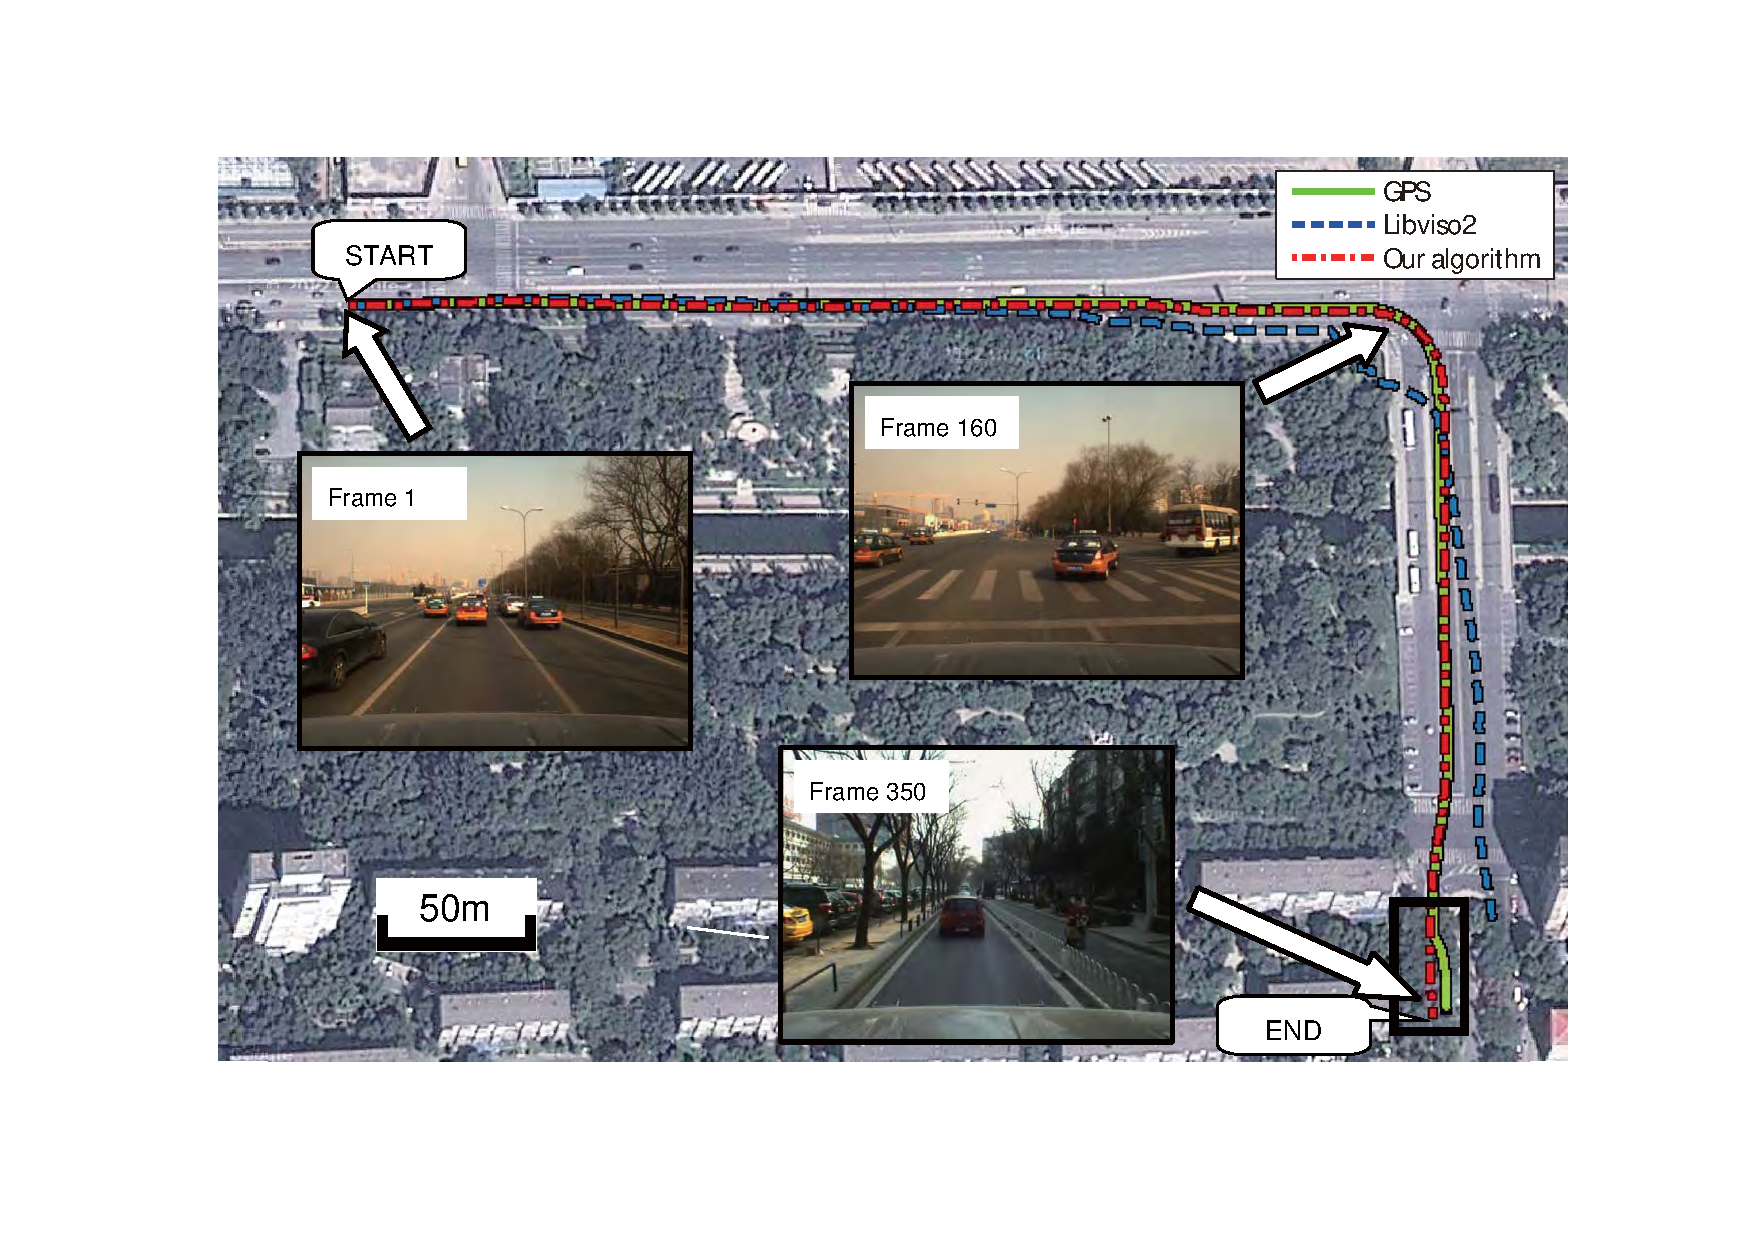
\includegraphics[width=0.9\linewidth]{source//Final//senario.pdf}
\caption{The scenario of the experiment. It takes two minutes driving about 600 meters with 350 frames taken from the camera on the roof of the vehicle. Green line is the trajectory got from the GPS/IMU system. Blue dash-line and red dash-dot-line denote for that of libviso2 and the proposed method. As the performance of GPS/IMU is not good at the end of the path, this part is ignored in validation.}
\label{fig:scenario}
\end{figure}

\begin{figure}[t]
\centering
    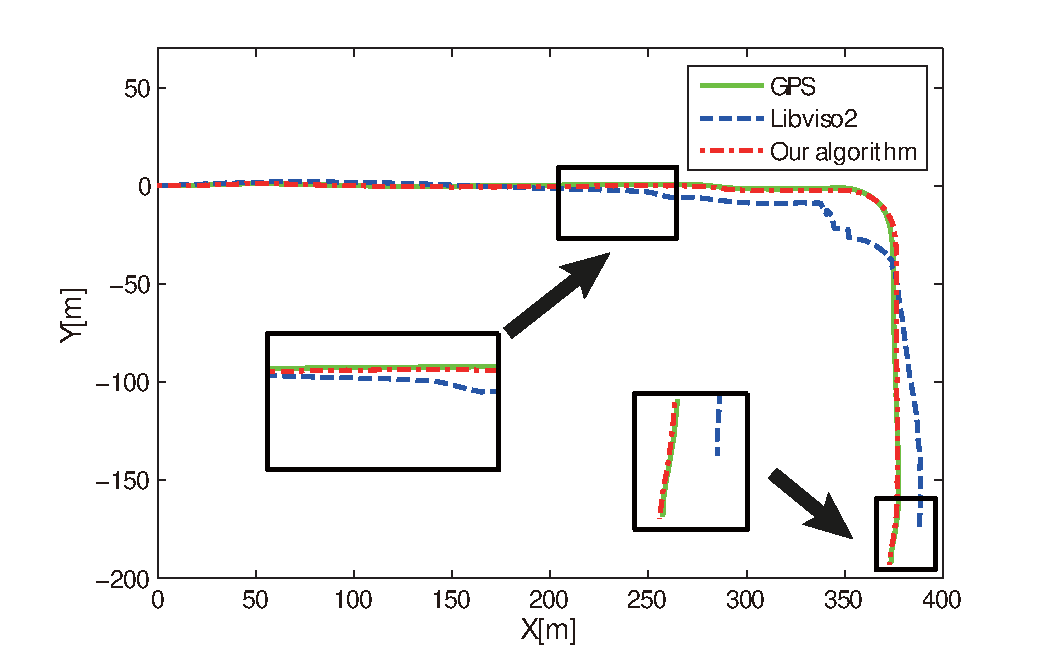
\includegraphics[width=1\linewidth]{source//Final//T_result.pdf}
\caption{The detail of positioning results in 2D space. The trajectories start at point (0,0) and green line, blue dash-line and red dash-dot-line represent those from GPS/IMU system, libviso2 and the proposed method.}
\label{fig:positions}
\end{figure}
\begin{figure}[t]
\centering
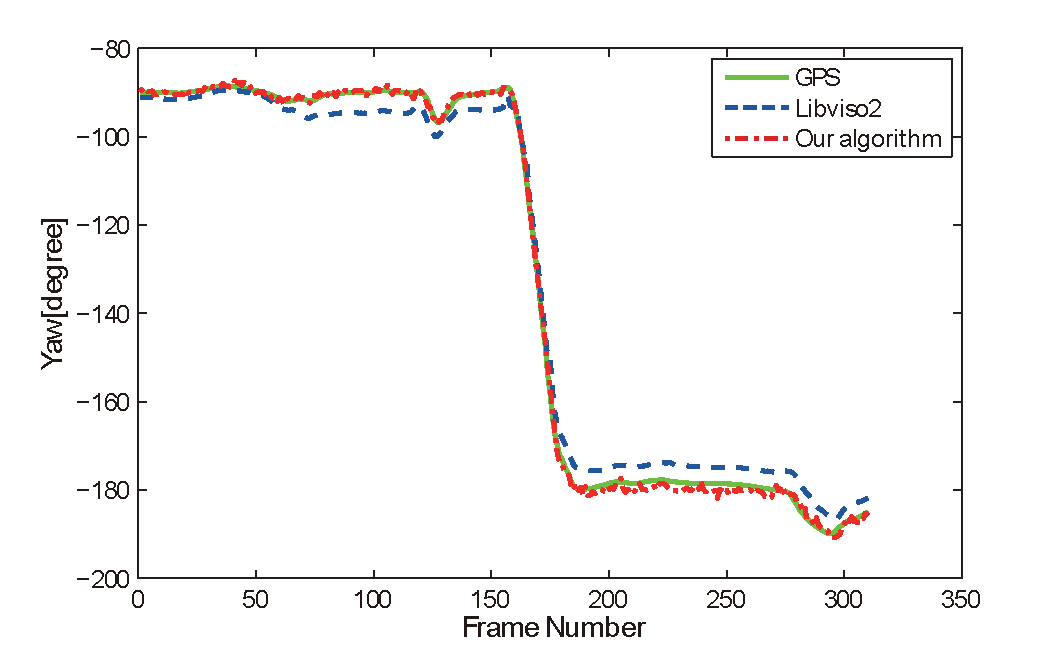
\includegraphics[width=0.95\linewidth]{source//Final//R_result.pdf}
\caption{The yaw results. Green line, blue dash-line and red dash-dot-line represent those from GPS/IMU system, libviso2 and the proposed method.}
\label{fig:yaw}
\end{figure}

In this experiment, we use the LSD method \cite{von2012lsd} to detect line segments from a monocular image, and subsequently extract road structural feature (RSF), which is used to locate the vehicle pose with a road map. We compare the performance with the monocular part of libviso2 \cite{Geiger11}\cite{Geiger2013Visual}, which is a popular visual odometry method, and GPS/IMU localization data. Vehicle trajectories of the three methods are visualized on a Google Map (start at(39.9754760, 116.3911050)) as shown in Fig. \ref{fig:scenario}, where the red dash-dot-line, blue dash-line and green line denote for that of the proposed method, libviso2 and GPS/IMU outputs. In the experimental site, the sky is open with few tall buildings, thus the GPS/IMU data is quite accurate in most cases. However, the performance of the GPS/IMU is somewhat affected by the trees at the end of the path, as shown in the "END" area in Fig. \ref{fig:scenario}, which is ignored in validation. Due to the interferences from environmental cars and the high dynamics of ego-vehicle's motion during its turn, a big error happened in vehicle pose estimation using libviso2 and the trajectories diverse after the ego-vehicle finished right turn. On the other hand, the proposed algorithm demonstrate much better result comparing to that of libviso2, where the red dash-dot-line (i.e. result of the proposed method) and the green line have nearly perfect matching. One of the major reason for this is that the proposed method use a map to constrain vehicle pose estimation, which provides a prior knowledge of the road directions. More details in positioning results are shown in Fig. \ref{fig:positions}, where only 310 frames used in validation because of the bad performance of the GPS/IMU system at the end of the travel.

Estimations of the vehicle heading are plotted in Fig. \ref{fig:yaw}. It can be found out that the result of the proposed method (red dash-dot-line) is much closer to GPS/IMU data (green line), while it shows some zigzags, reflecting poor local consistencies. The main reason for this zigzags could be considered that inter-frame matching is not included in the proposed framework, which sacrifices local consistencies of the result.

\begin{table}[t]
\caption{The position and rotation error}
\centering
\begin{tabular}{|r||c||c|}
\hline
&Mean Position Error(m) & Mean Rotation Error(deg)\\
\hline
libviso2 & $5.6426$ & $3.346$\\
\hline
our method & $0.5609$ & $0.779$\\
\hline
\end{tabular}
\label{table:Error_Result}
\end{table}

The result of average error of position and heading is shown in Table. \ref{table:Error_Result}. The errors of libviso2 and the proposed method are calculated compared with GPS/IMU result in each frame. Then the results are calculated by averaging the absolute value of the errors. It shown that the proposed algorithm performs better than libviso2.

In order to visualize the results, a map containing road structural features can be subsequently generated as shown in Fig. \ref{fig:lineProjection}, where the line features with road's longitude direction are projected. By manual classification, lane markings, road curbs, zebra zones are represented. In that case, after overlapping ego-vehicle's trajectory on the map, the interactive behaviors, such as lane changing maneuvers, can be identified directly.

\begin{figure*}
\centering
%\includegraphics[width=1\linewidth]{source//fig9.png}
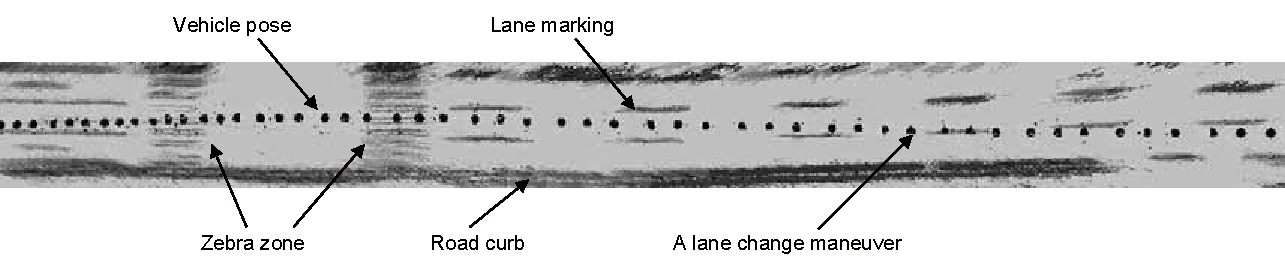
\includegraphics[width=1\linewidth]{source//Final//horizon_line.pdf}
\caption{The result of line segments projected onto horizontal plane. The line segments with road's longitude direction are projected. After manually marking the lines with lane markings, road curbs and zebra zones, a lane changing behavior can be identified.}
\label{fig:lineProjection}
\end{figure*}

Since the proposed method uses a 2D map, while libviso2 doesn't, it seems unfair to compare them. So another experiment has been done without the help of the map by assuming that our vehicle is driving in a straight road. It takes 4 minutes and 42 seconds driving about 3000 meters with 850 frames. The results are visualized on a Google Road Map (start at(39.9544800, 116.3031370)) as shown in Fig. \ref{fig:another_result}, where the red dash-dot-line, blue dash-line and green line denote for that of the proposed method, libviso2 and GPS/IMU outputs. The result of libviso2 is quit different from the GPS data after frame 412 because of the rotation error. Fig. \ref{fig:another_rotation_result} shows that on frame 419 and frame 619, the result of the yaw from libviso2 has two big jumps, which make the trajectory quit unusual. Since the road is non-strict straight, the result of our algorithm is a little different from the real trajectory after frame 400, where the direction of the road changes several degrees, as the GPS/IMU data shows in fig \ref{fig:another_rotation_result}.

\begin{figure}[t]
\centering
 \begin{minipage}[t]{0.48\linewidth}
    \centering
    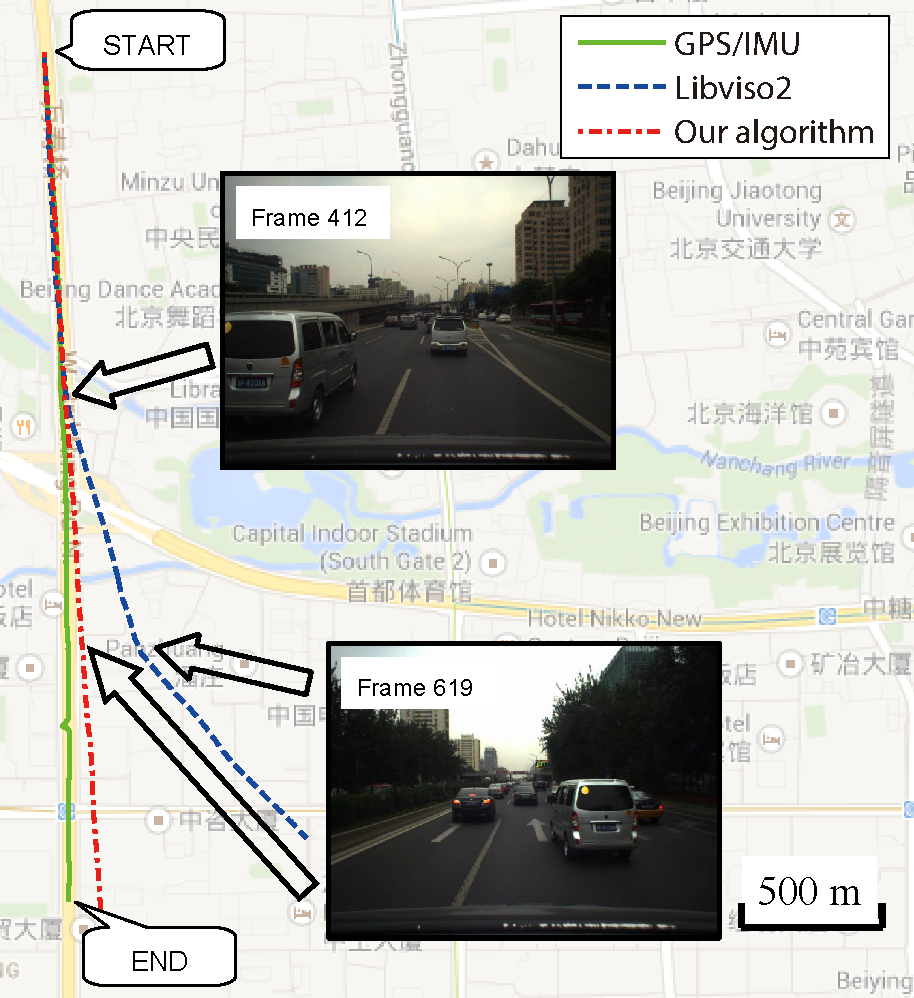
\includegraphics[width=1\textwidth]{source//Final//T_result_in_map_Frame200_1049.pdf}
    \label{fig:another_T_in_map}
  \end{minipage}%
  \hfill
 \begin{minipage}[t]{0.48\linewidth}
    \centering
    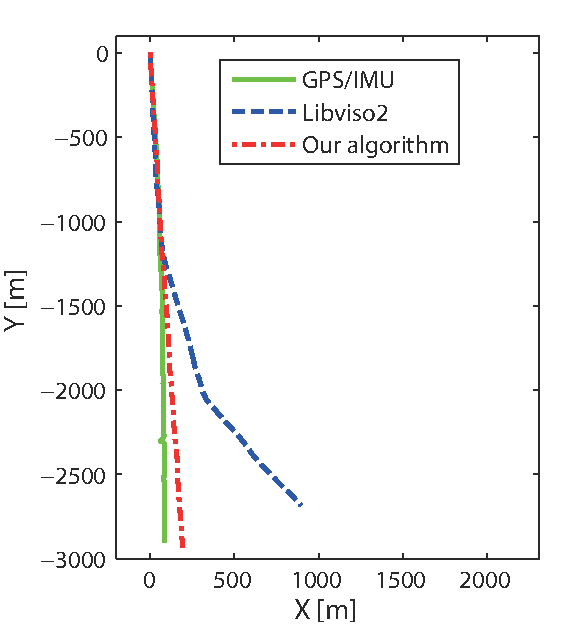
\includegraphics[width=1\textwidth]{source//Final//T_result_Frame200_1049.pdf}
    \label{fig:another_T_result}
  \end{minipage}%\
\caption{The positioning result of the other experiment. It takes 4 minutes and 42 seconds driving about 3000 meters with 850 frames taken from the camera on the roof of the vehicle. Green line, blue dash-line and red dash-dot-line represent the trajectories from GPS/IMU system, libviso2 and the proposed method.}
\label{fig:another_result}
\end{figure}

\begin{figure}[t]
\centering
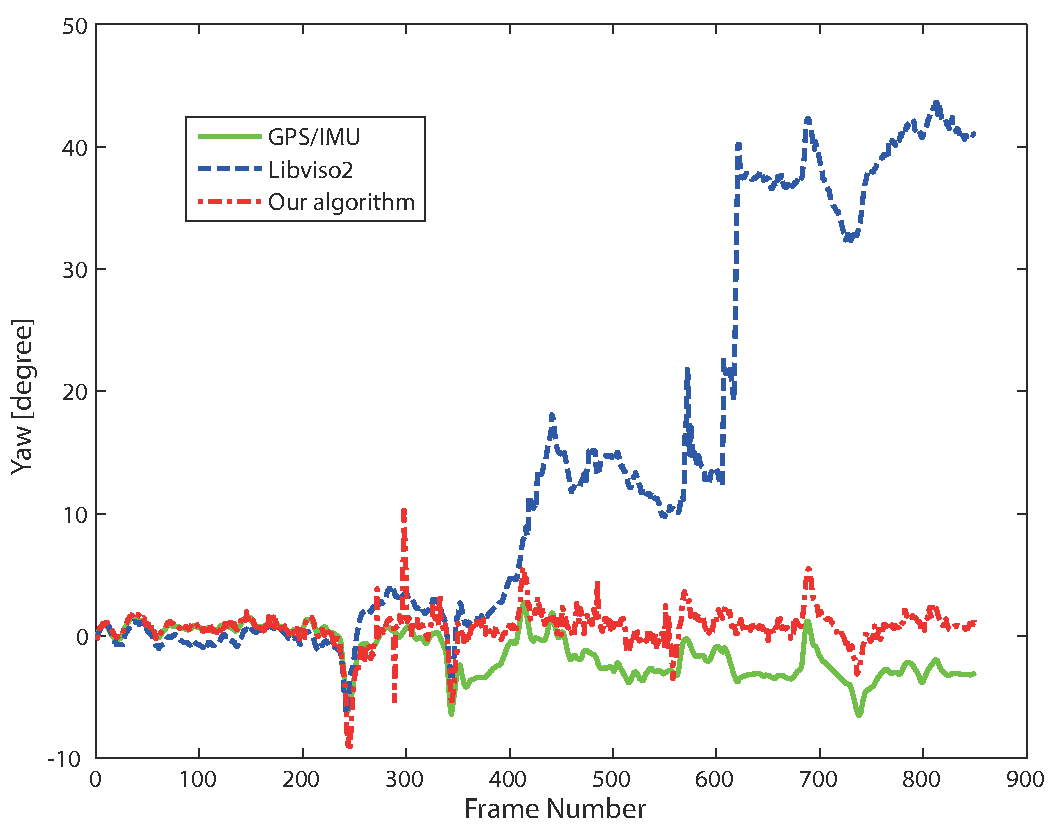
\includegraphics[width=0.9\linewidth]{source//Final//R_result_Frame200_1049.pdf}
\caption{The yaw result of the other experiment. Green line, blue dash-line and red dash-dot-line represent those from GPS/IMU system, libviso2 and the proposed method. The result of libviso2 shows two big errors on around frame 412 and frame 619.}
\label{fig:another_rotation_result}
\end{figure}

\section{Conclusions and Future Works}
In this research, a method using an on-board monocular camera is proposed to achieve precise localization at road lane level in structured road environments. In order to reduce the interference from dynamic traffics at the environment, so as to improve accuracy of a visual localization method, a road structural feature (RSF) is defined based on the line features with perpendicular directions and point features. The line features on such as lane markings, curbs, poles, building edges, etc., which are dominant, characterizes a structured road environment, and demonstrates the road's longitude, latitude and vertical directions.
A RSF-based visual localization method is proposed, where a prior knowledge to the environment, such as a 2D map with road-direction information, is implemented in a map-based localization framework, which predicts a RSF (or multiple RSFs at intersections) of the scene, and  estimates the vehicle pose after detecting the RSF from a monocular image with the predictions.
Experiments have been conducted using the video streams collected on major roads in central Beijing, which are structured and dynamic and a GPS/IMU data is recorded as a reference in validation.
The proposed algorithm shows better performance compared with a tradition visual odometry method.

While, the proposed algorithm have some limitations, which should be addressed in future work. As line segments are used to represent the features along three perpendicular axes of a structured road, the proposed algorithm works well on straight roads or turns. Extensions are needed for the scenes such as curved roads. On the other hand, the proposed work is utmost a position tracking algorithm, which requires a global localization to provide an initial position. It could be implemented as an assistant for GPS based localization, which will also be addressed in future work.

\bibliographystyle{IEEEtran}
\bibliography{IEEEabrv,IROS2013}

\end{document}
